\section{Mínimos cuadrados}

\subsection{}

{\nologo
\begin{frame}\frametitle{Introducción}


\begin{figure}
	\centering
	\begin{subfigure}[b]{0.27\textwidth}
		
\includegraphics[width=\textwidth]{imagenes/Piazzi}
%		\caption{Giuseppe Piazzi}
	\end{subfigure}
	\hspace{1.5cm}
%	\hfill
	~ %add desired spacing between images, e. g. ~, \quad, \qquad, \hfill etc. 
	%(or a blank line to force the subfigure onto a new line)
	\begin{subfigure}[b]{0.23\textwidth}
		
\includegraphics[width=\textwidth]{imagenes/Cerere}
%		\caption{Cubierta del libro de Piazzi \textit{Della scoperta del nuovo pianeta Cerere Ferdinandea}}
	\end{subfigure}
%	\caption{Pictures of animals}\label{fig:animals}
\end{figure}


\begin{defi}{}\justifying
	El 1 de enero de 1801, mientras inspeccionaba una región de la constelación de Tauro, 
	el astrónomo italiano Giuseppe Piazzi observó una pequeña ``estrella'' que nunca antes había
	sido divisada. Después de muchas observaciones, Piazzi y otros astrónomos notaron que la
	``estrella'' se movía y concluyeron que se trataba de un ``planeta'' (en realidad era un asteroide).
	El nuevo ``planeta'' despareció completamente en el otoño de 1801. Los astrónomos más reconocidos 
	de la época se unieron a la búsqueda para reubicar el ``planeta'' perdido, pero todos sus 
	esfuerzos fueron en vano.
\end{defi}	

\end{frame}
}

%%------------------------------------------------------------------------------------------------------

\subsection{}

{\nologo
\begin{frame}\frametitle{Introducción}
	
	
	\begin{figure}
		\centering
		\begin{subfigure}[b]{0.27\textwidth}
			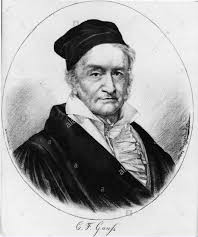
\includegraphics[width=\textwidth]{imagenes/Gauss}
			%		\caption{Giuseppe Piazzi}
		\end{subfigure}
		\hspace{1.5cm}
		%	\hfill
		~ %add desired spacing between images, e. g. ~, \quad, \qquad, \hfill etc. 
		%(or a blank line to force the subfigure onto a new line)
		\begin{subfigure}[b]{0.23\textwidth}
			
\includegraphics[width=\textwidth]{imagenes/Cerere}
			%		\caption{Cubierta del libro de Piazzi \textit{Della scoperta del nuovo pianeta Cerere Ferdinandea}}
		\end{subfigure}
		%	\caption{Pictures of animals}\label{fig:animals}
	\end{figure}
	
	\begin{defi}{}\justifying
		En septiembre de 1801 Carl F. Gauss decidió asumir el desafío de encontrar el ``planeta'' perdido. 
		Gauss consideró una órbita elíptica en lugar de una circular como habían asumido los demás y desarrolló
		el método de \textit{mínimos cuadrados}. En diciembre Gauss ya había resuelto el problema y reportó sus
		resultados a la comunidad científica, no solo con la posición del ``planeta'' en ese momento, sino 
		también con todas sus posiciones futuras. Los astrónomos dirigieron sus telescopios al cielo y encontraron
		al ``planeta'' exactamente donde Gauss lo había pronosticado. El ``planeta'' recibió el nombre de \textit{Ceres}.
	\end{defi}	
	
\end{frame}
}

%%------------------------------------------------------------------------------------------------------

\subsection{}

{\nologo
\begin{frame}\frametitle{Espacio renglón y espacio columna de una matriz}
	
	\begin{columns}[c]
		\begin{column}{1.15\textwidth}
			\[
			\begin{array}{@{\hspace{0.1\tabcolsep}}c@{\hspace{2\tabcolsep}}c@{\hspace{2\tabcolsep}}c@{\hspace{0.1\tabcolsep}}}
			\text{\textbf{Matriz }} A & \text{\textbf{Vectores renglón de }} A & \text{\textbf{Vectores columna de} } A \\[-8mm] 
			{\left(
				\begin{array}{@{\hspace{0.1\tabcolsep}}c@{\hspace{1.5\tabcolsep}}c@{\hspace{1.5\tabcolsep}}c@{\hspace{1.5\tabcolsep}}c@{\hspace{0.1\tabcolsep}}}
				a_{11} & a_{12} & \cdots & a_{1n} \\[1mm]
				a_{21} & a_{22} & \cdots & a_{2n} \\[1mm]
				\vdots & \vdots &        & \vdots \\[0mm]
				a_{m1} & a_{m2} & \cdots & a_{mn} \\[1mm]
				\end{array}
				\right)
				\atop		
			}
			& 
			\begin{array}{@{\hspace{0.1\tabcolsep}}c@{\hspace{0.5\tabcolsep}}c@{\hspace{0.5\tabcolsep}}l@{\hspace{0.1\tabcolsep}}}
			\mathbf{r}_1 & = & (a_{11},a_{12},\hdots, a_{1n})\\[1mm]
			\mathbf{r}_2 & = & (a_{21},a_{22},\hdots, a_{2n})\\
			& \vdots & \\[1mm]
			\mathbf{r}_m  & = & (a_{m1},a_{m2},\hdots, a_{mn})\\[1.1cm]
			\end{array}
			& 
			{
				\begin{array}{@{\hspace{0.1\tabcolsep}}c@{\hspace{1.3\tabcolsep}}c@{\hspace{1.3\tabcolsep}}c@{\hspace{1.3\tabcolsep}}c@{\hspace{0.1\tabcolsep}}}\\[8mm]
				\underbrace{\!\!
					\left(
					\begin{array}{@{\hspace{0.1\tabcolsep}}c@{\hspace{0.1\tabcolsep}}}
					a_{11}\\[1mm]
					a_{21}\\[1mm]
					\vdots \\[0mm]
					a_{m1}
					\end{array}
					\right)
					\!\!}_{\mathbf{c}_1}
				& 
				\underbrace{\!\!
					\left(
					\begin{array}{@{\hspace{0.1\tabcolsep}}c@{\hspace{0.1\tabcolsep}}}
					a_{12}\\[1mm]
					a_{22}\\[1mm]
					\vdots \\[0mm]
					a_{m2}
					\end{array}
					\right)
					\!\!}_{\mathbf{c}_2}
				& 
				\cdots
				& 
				\underbrace{\!\!
					\left(
					\begin{array}{@{\hspace{0.1\tabcolsep}}c@{\hspace{0.1\tabcolsep}}}
					a_{1n}\\[1mm]
					a_{2n}\\[1mm]
					\vdots \\[0mm]
					a_{mn}
					\end{array}
					\right)
					\!\!}_{\mathbf{c}_n}
				\end{array}
				\atop
			}				
			\end{array}		
			\]
		\end{column}
	\end{columns}
	
	\vspace{-4mm}
	
	
	% \begin{defi}{\textbf{Definición 1}}
	\begin{defi}{}
		Sea $A$ una matriz ${\color{blue}m}\times {\color{red}n}$.
		\begin{enumerate}
			\item[\labelname{$a$}] El \textbf{\textit{espacio renglón}} de $A$ es el subespacio de $\r^{\color{red}n}$ generado por los renglones de $A$:
			\[
			R_A = \text{gen}\, \{ \mathbf{r}_1, \mathbf{r}_2, \hdots,\mathbf{r}_{\color{blue}m} \}
			\]
			
			\smallskip
			\item[\labelname{$b$}] El \textbf{\textit{espacio columna}} de $A$ es el subespacio de $\r^{\color{blue}m}$ generado por las columnas de $A$:
			\[
			C_A = \text{gen}\, \{ \mathbf{c}_1, \mathbf{c}_2, \hdots,\mathbf{c}_{\color{red}n} \}
			\]
		\end{enumerate}
	\end{defi}	
	
\end{frame}
}

%%------------------------------------------------------------------------------------------------------
\subsection{}

\begin{frame}\frametitle{Espacio renglón y espacio columna de una matriz}
		
	\begin{ej}{\textbf{Ejemplo 1}}
		Considere la matriz
		\[
		A = 
		\left(
		\begin{array}{ccc}
		1 & 2 & 0 \\[1mm]
		0 & 0 & 1\\[1mm]
		0 & 0 & 0\\[1mm]
		0 & 0 & 0\\[1mm]
		\end{array}
		\right)
		\]
		Halle
		
		\vspace{-2mm}
		\begin{multicols}{4}
			\begin{enumerate}\justifying
				\item[\labelname{$a$}] $C_A$
				\item[\labelname{$b$}] $C_{A^T}$
				\item[\labelname{$d$}] $N_A$
				\item[\labelname{$d$}] $N_{A^T}$
			\end{enumerate}
		\end{multicols}		
	
		\vspace{-3mm}	
	\end{ej}
	\textit{Solución}.
	
\end{frame}

%%------------------------------------------------------------------------------------------------------

\subsection{}

\begin{frame}\frametitle{Propiedades de los espacios fundamentales de una matriz}
	
	\begin{prop}{\textbf{Propiedad 1}}
		\justifying
		Si $A$ es una matriz ${\color{blue}m}\times {\color{red}n}$, entonces
		\begin{enumerate}\justifying
			\item[\labelname{$a$}] $C_A$ y $N_{A^T}$ son subespacios ortogonales de $\r^{\color{blue}m}$.
			\item[\labelname{$b$}] $C_{A^T}$ y $N_{A}$ son subespacios ortogonales de $\r^{\color{red}n}$.
			\item[\labelname{$c$}] ${\left(C_A\right)}^{\perp} = N_{A^T}$.
			\item[\labelname{$d$}] ${\left(C_{A^T}\right)}^{\perp} = N_{A}$.
		\end{enumerate}
	\end{prop}		
	
\end{frame}

%%------------------------------------------------------------------------------------------------------

\subsection{}

\begin{frame}\frametitle{Espacio renglón y espacio columna de una matriz}
	
	\begin{ej}{\textbf{Ejemplo 2}}
		¿Cómo hallar una recta $y=mx+b$ que ``mejor se ajuste'' a los puntos 
		\[
			(1,0),\  (2,1) \ \ \text{y} \ \ (3,3)?
		\]
	\end{ej}
	\textit{Solución}.
	
\end{frame}

%%------------------------------------------------------------------------------------------------------

\subsection{}

{\nologo
\begin{frame}\frametitle{Aproximación por mínimos cuadrados}
		
	\begin{ejem}{\textbf{Problema de mínimos cuadrados}}
		\justifying
		Sea $A$ una matriz $m\times n$ y $\mathbf{b}$ un vector en $\r^m$. Hallar un vector $\mathbf{x}$ en $\r^n$
		que minimice a
		\begin{equation}\label{eq:error}
			\left\Vert A\mathbf{x} - \mathbf{b} \right\Vert. 
		\end{equation}					
	\end{ejem}

	\begin{alertblock}{\textbf{Observación 1}}
		\begin{itemize}
			\item[\labelname{$a$}] $\left\Vert A\mathbf{x} - \mathbf{b} \right\Vert \geq 0 $ para todo $\mathbf{x}$ en $\r^n$.
			\item[\labelname{$b$}] El valor mínimo posible de la expresión \eqref{eq:error} es 
			$\left\Vert A\mathbf{x} - \mathbf{b} \right\Vert = 0 $ y en tal caso
			\[
				A\mathbf{x} = \mathbf{b}.
			\]
			\item[\labelname{$c$}] El sistema $A\mathbf{x} = \mathbf{b}$ es consistente si y sólo si $\mathbf{b}$ está en $C_A$.
			\item[\labelname{$d$}] Si $\left\Vert A\mathbf{x} - \mathbf{b} \right\Vert > 0 $, entonces
			\[
				A\mathbf{x} \neq \mathbf{b}.
			\]
			\item[\labelname{$e$}] Estamos interesados en resolver el \textit{problema de mínimos cuadrados} 
			en el caso en que el sistema $A\mathbf{x} = \mathbf{b}$ es inconsistente (no tiene solución).
			\item[\labelname{$f$}] El sistema $A\mathbf{x} = \mathbf{b}$ es inconsistente si y sólo si 
			$\mathbf{b}$ no está en $C_A$.
		\end{itemize}
	\end{alertblock}
	
\end{frame}
}

%%------------------------------------------------------------------------------------------------------

\subsection{}

\begin{frame}%\frametitle{Mínimos cuadrados}
	
	\begin{ejem}{\textbf{Problema de mínimos cuadrados}}
		\justifying
		Sea $A$ una matriz $m\times n$ y $\mathbf{b}$ un vector en $\r^m$. Hallar un vector $\mathbf{x}$ en $\r^n$
		que minimice a
		\begin{equation}\tag{1}
		\left\Vert A\mathbf{x} - \mathbf{b} \right\Vert. 
		\end{equation}					
	\end{ejem}
	\textit{Solución}.
	
	\vspace{-3mm}
	\begin{columns}
		\begin{column}{0.55\textwidth}
			\begin{itemize}		
				\item Suponemos que $\mathbf{b}$ no está en $C_A$.
				
				\vspace{2mm}
				\item $A\mathbf{x}$ está en $C_A$ para todo $\mathbf{x}$ en $\r^n$.
				
				\vspace{2mm}
				\item Buscamos un vector $A\mathbf{\widehat{x}}$ en $C_A$ que esté lo ``más próximo posible'' a $\mathbf{b}$.
			\end{itemize}
		\end{column}
		\begin{column}{0.35\textwidth}  %%<--- here
			
			\vspace{-2mm}
			\begin{figure}
				\centering
				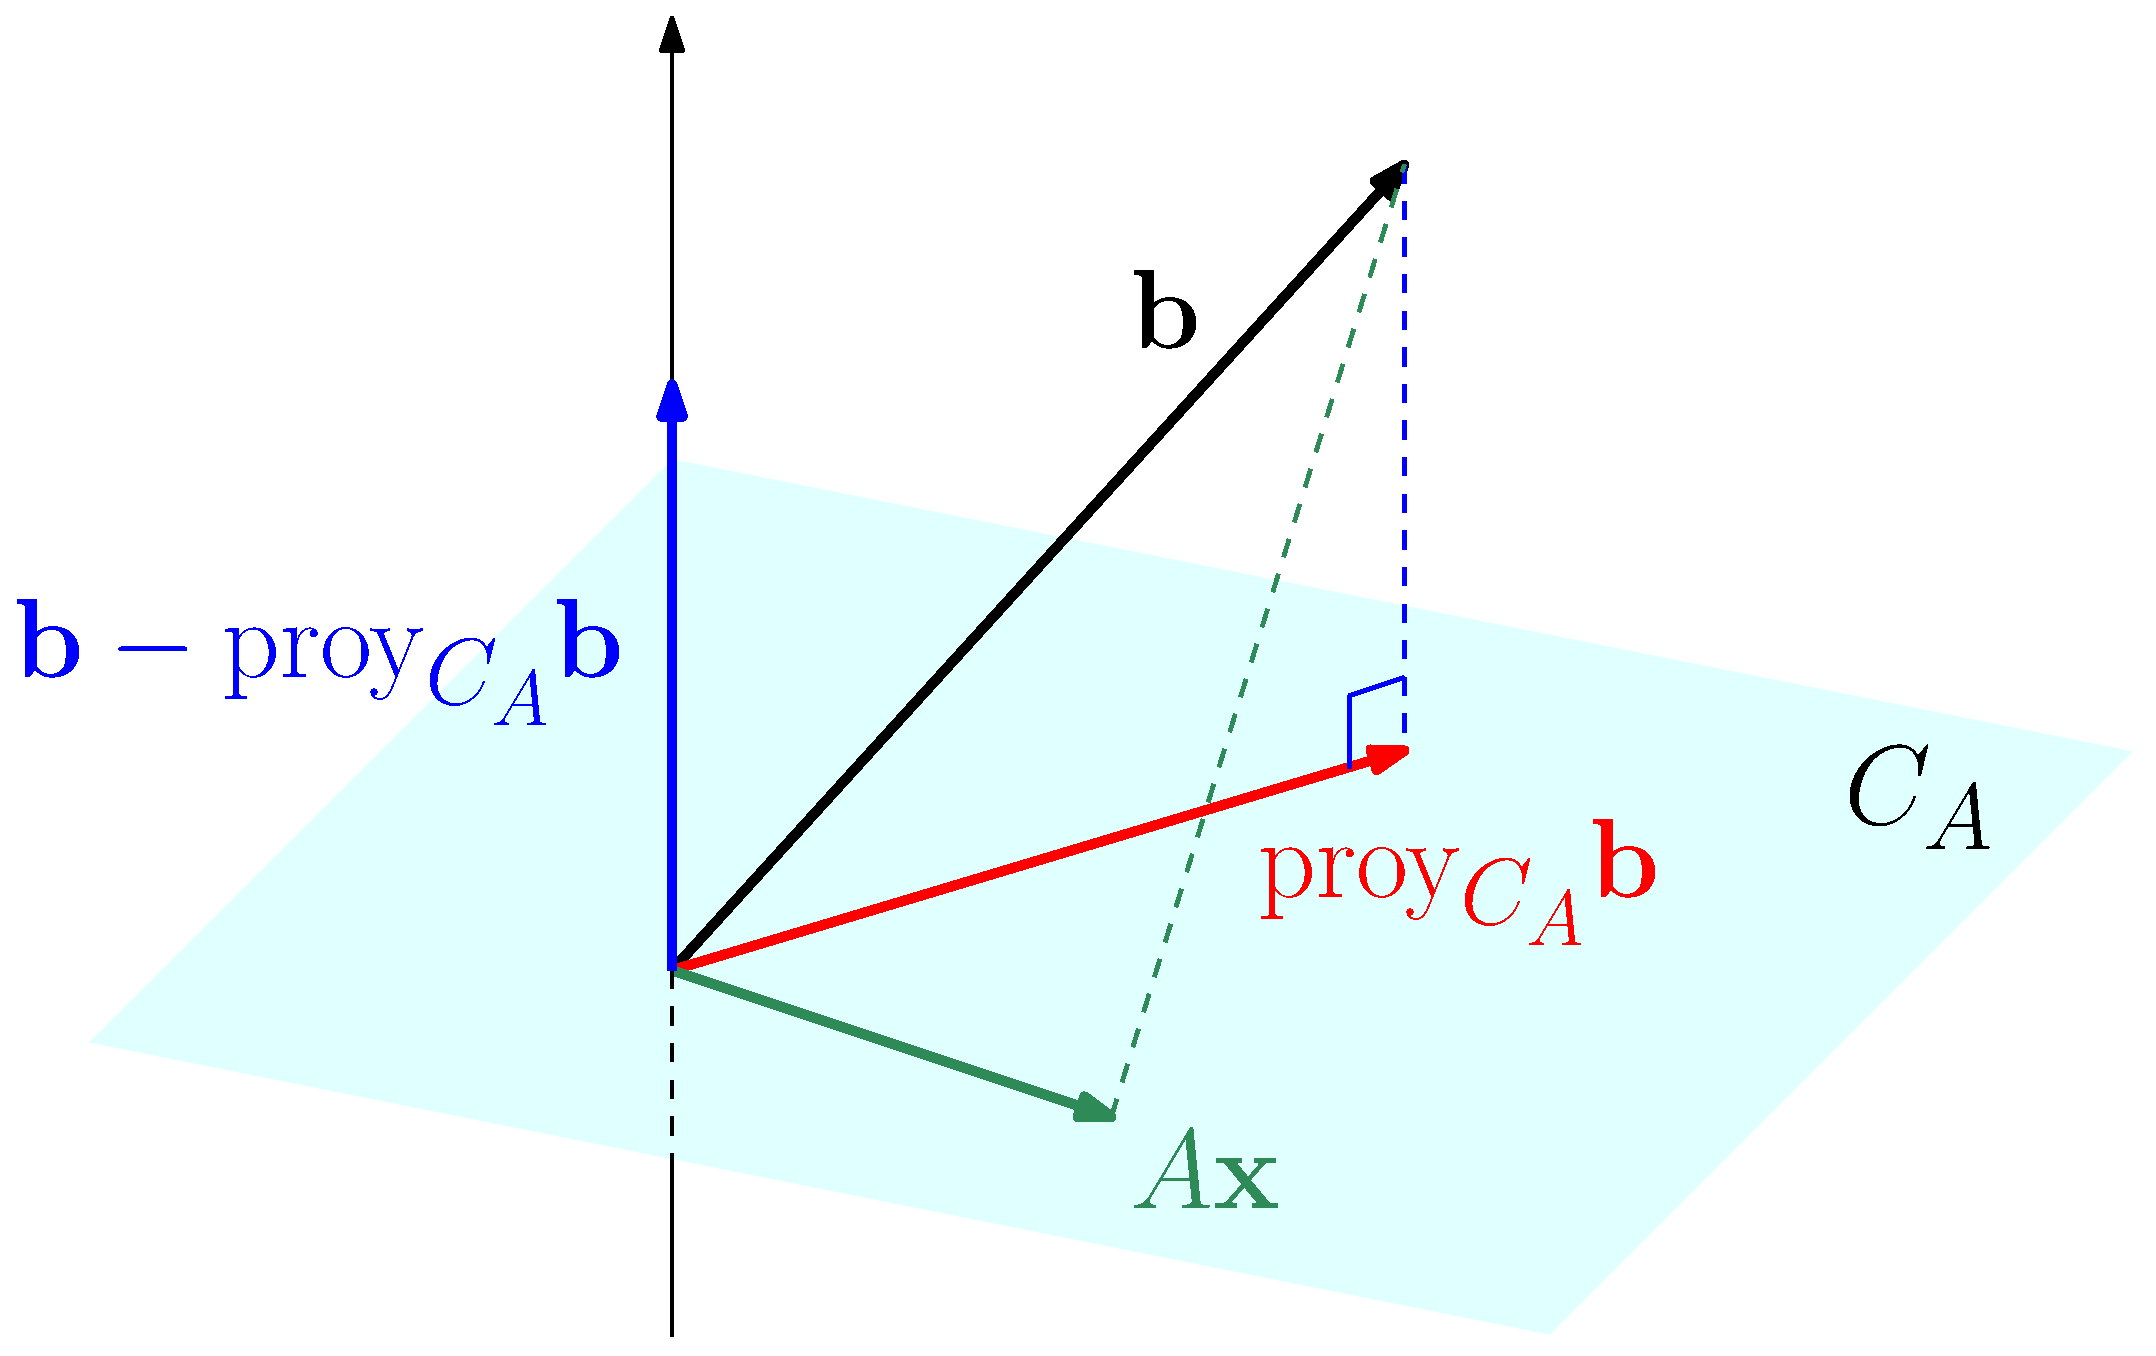
\includegraphics[width=3.5cm]{imagenes/minimos.eps}
				{\scriptsize  $\Vert \mathbf{b}-\text{proy}_{C_A}\mathbf{b}  \Vert \leq \Vert \mathbf{b} - A\mathbf{x}\Vert $}
				%\caption{$ \Vert \mathbf{b}-\text{proy}_{C_A}\mathbf{b}  \Vert \leq \Vert \mathbf{b} - A\mathbf{x}\Vert $}
			\end{figure}
		\end{column}
	\end{columns}
	
	\vspace{0mm}
	\begin{itemize}		
		\item El vector $A\mathbf{\widehat{x}}$ en $C_A$ ``más próximo'' a $\mathbf{b}$ es		
		\[
			A\mathbf{\widehat{x}} = \text{proy}_{C_A} \mathbf{b}.
		\]

		%\vspace{-0mm}
		%\item El vector $A\mathbf{\widehat{x}}-\mathbf{b}$ es ortogonal a $C_A$.

		\vspace{1mm}
		\item El vector $A\mathbf{\widehat{x}}-\mathbf{b}$ está en ${\left(C_A\right)}^{\perp} = N_{A^T}$ y por tanto
		
		\vspace{-0mm}
		\[
		\begin{array}{rcl}
		A^T \left(A\mathbf{\widehat{x}} - \mathbf{b} \right) & =               & \mathbf{0} \\[1mm]
		A^TA\,\mathbf{\widehat{x}} - A^T\mathbf{b} & =               & \mathbf{0} \\[1mm]
		{\color{red} A^TA\, \mathbf{\widehat{x}} } & {\color{red} =} & {\color{red} A^T\mathbf{b}} 
		\end{array}
		\]
	\end{itemize}
		
\end{frame}

%%------------------------------------------------------------------------------------------------------

\subsection{}

{\nologo
\begin{frame}\frametitle{Aproximación por mínimos cuadrados}
	
	\begin{prop}{\textbf{Propiedad 1}}
		\justifying
		Si $A$ es una matriz $m\times n$ de rango $n$, entonces $A^TA$ es una matriz $n\times n$ 
		invertible y el \textit{problema de mínimos cuadrados} tiene una única 
		solución que se obtiene al resolver el sistema
		\begin{equation}\label{eq:minimos}
			A^TA\, \mathbf{x} = A^T\mathbf{b}.
		\end{equation}
	\end{prop}		
	
		\begin{alertblock}{\textbf{Observación 1}}
		\begin{itemize}\justifying
			\item[\labelname{$a$}] El sistema de ecuaciones lineales \eqref{eq:minimos} recibe el 
			nombre de \textit{ecuaciones normales} del problema de mínimos cuadrados 
			$A\mathbf{x} = \mathbf{b}$.
			\item[\labelname{$b$}] El problema de mínimos cuadrados siempre tiene al menos una solución.
			\item[\labelname{$c$}] Bajo las hipótesis de la propiedad 1, el problema de mínimos cuadrados 
			tiene exactamente una solución y está dada por
			\[
				\mathbf{x} = \left( A^TA \right)^{-1} A^T \mathbf{b}.
			\]
		\end{itemize}
	\end{alertblock}

\end{frame}
}

%%------------------------------------------------------------------------------------------------------

\subsection{}

\begin{frame}\frametitle{Aproximación por mínimos cuadrados}
	
	\begin{ej}{\textbf{Ejemplo 3}}
		Encuentre la solución del problema de mínimos cuadrados para los puntos de datos
		\[
		(1,0),\  (2,1) \ \ \text{y} \ \ (3,3)
		\]
		del ejemplo 2.
	\end{ej}
	\textit{Solución}.
	
\end{frame}

%%------------------------------------------------------------------------------------------------------

\subsection{}

{\nologo
\begin{frame}\frametitle{Procedimiento de aproximación lineal por mínimos cuadrados}
	
	\vspace{-3mm}
	\begin{ejem}{\textbf{Procedimiento 1}}
		\justifying
		El procedimiento para determinar la recta de mínimos cuadrados 
		
		\vspace{-2mm}
		\[
			y = c_0 + c_1 x
		\] 
		
		\vspace{-2mm}
		para los datos 
		\[
			(x_1, y_1 ), (x_2, y_2 ), \hdots ,(x_n , y_n ),
		\]
		 donde por lo menos dos de las $x_i$ son diferentes, es el siguiente.
		\begin{enumerate}\justifying
			\item Defina
					\[						
						A = 
						\left(
						\begin{array}{cc}
						1 & x_1 \\[1mm]
						1 & x_2 \\[1mm]
						\vdots & \vdots \\[1mm]
						1 & x_n \\[1mm]
						\end{array}
						\right),
						\quad
						\mathbf{x} = 
						\left(
						\begin{array}{c}
						c_0 \\[1mm]
						c_1 
						\end{array}
						\right)
						\qquad \text{y} \qquad 
						\mathbf{b} = 
						\left(
						\begin{array}{c}
						y_1  \\[1mm]
						y_2 \\[1mm]
						\vdots \\[1mm]
						y_n\\[1mm]
						\end{array}
						\right).
					\]
			\item Resuelva el sistema de ecuaciones normales
				\[
					A^TA\, \mathbf{x} = A^T\mathbf{b}
				\]		
				para $\mathbf{x}$, mediante eliminación de mediante Gauss-Jordan.
		\end{enumerate}
	\end{ejem}		
	
\end{frame}
}

%%------------------------------------------------------------------------------------------------------

\subsection{}

\begin{frame}\frametitle{Aproximación polinomial por mínimos cuadrados}
	
	\begin{ej}{\textbf{Ejemplo 4}}\justifying
		Encuentre la parábola que ofrezca la mejor aproximación por mínimos cuadrados a los
		puntos
		\[	
			(-1, 1),\ (0, -1),\ (1, 0) \ \ \text{y} \ \ (2, 2).
		\]
	\end{ej}
	\textit{Solución}.
	
\end{frame}

%%------------------------------------------------------------------------------------------------------

\subsection{}

{\nologo
\begin{frame}\frametitle{Procedimiento de aproximación polinomial por mínimos cuadrados}
	
	\vspace{-3mm}
	\begin{ejem}{\textbf{Procedimiento 2}}
		\justifying
		El procedimiento para determinar el polinomio por mínimos cuadrados
		
		\vspace{-2mm}
		\[
			y = c_0 + c_1 x + \cdots + c_{m-1} x^{m-1} + c_m x^m   
		\] 
		
		\vspace{-1mm}
		que mejor se ajusta a los datos
		\[
		(x_1, y_1 ), (x_2, y_2 ), \hdots ,(x_n , y_n ),
		\]
		donde $m\leq n-1$ y por lo menos $m + 1$ de los $x_i$ son distintos, es el siguiente.
		

		\begin{enumerate}\justifying
			\item Defina
			
			\vspace{-4mm}
			\[						
			A = 
			\left(
			\begin{array}{ccccc}
				1 & x_1 & \cdots & x_1^{m-1} & x_1^m \\[1mm]
				1 & x_2 & \cdots & x_2^{m-1} & x_2^m \\[1mm]
				\vdots & \vdots &  & \vdots & \vdots \\[1mm]
				1 & x_n & \cdots & x_n^{m-1} & x_n^m \\[1mm]
			\end{array}
			\right),
			\ \
			\mathbf{x} = 
			\left(
			\begin{array}{c}
			c_0 \\[1mm]
			c_1 \\[1mm]
			\vdots \\[1mm]
			c_m 
			\end{array}
			\right)
			\ \ \text{y} \ \ 
			\mathbf{b} = 
			\left(
			\begin{array}{c}
			y_1  \\[1mm]
			y_2 \\[1mm]
			\vdots \\[1mm]
			y_n\\[1mm]
			\end{array}
			\right).
			\]
			
			\vspace{0mm}
			\item Resuelva para $\mathbf{x}$ el sistema de ecuaciones normales
			\[
			A^TA\, \mathbf{x} = A^T\mathbf{b}
			\]		
		\end{enumerate}
	\end{ejem}		
	
\end{frame}
}

%%------------------------------------------------------------------------------------------------------

\subsection{}

\begin{frame}%\frametitle{Aproximación por mínimos cuadrados}
	
	\begin{ej}{\textbf{Ejemplo 5}}\justifying
		La  tabla\footnote{\href{https://en.wikipedia.org/wiki/COVID-19_pandemic_in_Colombia\#March}{\color{blue}https://en.wikipedia.org/wiki/COVID-19\_pandemic\_in\_Colombia}} presenta el número de infectados por SARS-CoV-2 en Colombia, durante los primeros días de la pandemia, en 
		marzo de 2020. Si supone un modelo de crecimiento exponencial, encuentre la tasa de crecimiento relativa y estime 
		el número de infectados para el 25 de marzo.
		
		\begin{center}
			\renewcommand{\arraystretch}{1.3}
			\begin{tabular}{|>{\columncolor{gray!20}}c|c|c|c|c|c|c|}\hline
				      Día & $13$ & $14$ & $15$ & $16$ & $17$ & $18$\\ \hline
				Infectados & $16$ & $24$ & $45$ & $57$ & $75$ & $102$ \\ \hline
			\end{tabular}
		\end{center}
		% https://www.wolframalpha.com/input/?i=exponential+fit+%7B%7B13%2C+16%7D%2C+%7B14%2C+24%7D%2C+%7B15%2C+45%7D%2C+%7B16%2C+57%7D%2C+%7B17%2C+75%7D%2C+%7B18%2C+102%7D%7D

		\vspace{-1mm}
	
	\end{ej}
	\textit{Solución}.
	
\end{frame}
